\documentclass[UTF8,a4paper,12pt]{ctexart}

\usepackage[margin=2.2cm]{geometry}
\usepackage{graphicx}
\usepackage{booktabs}
\usepackage{float}
\usepackage{subcaption}
\usepackage{amsmath}
\usepackage{xcolor}
\usepackage{listings}
\usepackage{hyperref}

\graphicspath{{./}{outputs/}}

\hypersetup{
  colorlinks=true,
  linkcolor=blue,
  urlcolor=blue,
  citecolor=blue
}

\lstdefinestyle{py}{
  language=Python,
  basicstyle=\ttfamily\small,
  keywordstyle=\color{blue!70!black},
  commentstyle=\color{green!40!black},
  stringstyle=\color{orange!60!black},
  numbers=left,
  numberstyle=\tiny\color{gray},
  stepnumber=1,
  numbersep=8pt,
  frame=single,
  breaklines=true,
  tabsize=4,
  showstringspaces=false
}

\title{视频图像处理实验报告\\第二次作业：图像配准}
\author{姓名：\underline{\hspace{3cm}} \quad 学号：\underline{\hspace{3cm}}}
\date{\today}

\begin{document}
\maketitle
\tableofcontents
\newpage

\section{实验目的}
\begin{enumerate}
  \item 理解图像配准（Image Registration）的基本流程。
  \item 掌握从两幅图像中提取对应点并估计单应矩阵 $H$ 的方法。
  \item 完成图像透视变换并输出配准结果图。
  \item 通过叠加图与误差热力图评估配准效果。
\end{enumerate}

\section{实验环境与数据}
\subsection{实验环境}
\begin{itemize}
  \item 操作系统：Windows
  \item 编程语言：Python 3
  \item 主要库：NumPy、Pillow、Matplotlib、scikit-image
\end{itemize}

\subsection{实验数据}
\begin{itemize}
  \item \texttt{Image A.jpg}（固定图像，Fixed）
  \item \texttt{Image B.jpg}（待配准图像，Moving）
\end{itemize}

\section{实验任务}
根据题目要求，在两幅图像中随机选取 7 个对应点，计算两幅图像之间的转换矩阵 $H$，并输出转换后的图像。

\section{实验原理}
\subsection{单应变换模型}
对于同一平面或近似平面场景，图像间可用单应矩阵描述：
\begin{equation}
\begin{bmatrix}
x'\\y'\\1
\end{bmatrix}
\sim
\mathbf{H}
\begin{bmatrix}
x\\y\\1
\end{bmatrix},
\quad
\mathbf{H}\in\mathbb{R}^{3\times3}
\end{equation}
其中 $\sim$ 表示齐次坐标下相等（相差一个非零尺度因子）。

\subsection{特征匹配与 RANSAC}
\begin{enumerate}
  \item 使用 ORB 提取关键点与描述子；
  \item 进行描述子匹配得到候选对应点；
  \item 用 RANSAC 剔除误匹配，保留几何一致的内点；
  \item 在内点中随机取 7 对点估计 $\mathbf{H}$。
\end{enumerate}

\subsection{结果评估}
\begin{itemize}
  \item 使用配准后的图像与固定图像做半透明叠加，观察结构对齐程度；
  \item 使用绝对差热力图观察局部误差分布；
  \item 使用内点重投影 RMSE 作为数值指标。
\end{itemize}

\section{关键代码}
\subsection{ORB 特征提取与匹配}
\begin{lstlisting}[style=py]
def detect_and_match_points(fixed_gray, moving_gray):
    orb_fixed = feature.ORB(n_keypoints=3000, fast_threshold=0.07)
    orb_moving = feature.ORB(n_keypoints=3000, fast_threshold=0.07)
    orb_fixed.detect_and_extract(fixed_gray)
    orb_moving.detect_and_extract(moving_gray)
    matches = feature.match_descriptors(
        orb_fixed.descriptors,
        orb_moving.descriptors,
        cross_check=True,
        max_ratio=0.8
    )
    fixed_pts = np.fliplr(orb_fixed.keypoints[matches[:, 0]])
    moving_pts = np.fliplr(orb_moving.keypoints[matches[:, 1]])
    return fixed_pts, moving_pts
\end{lstlisting}

\subsection{RANSAC 过滤误匹配}
\begin{lstlisting}[style=py]
model, inliers = ransac(
    (moving_pts, fixed_pts),
    transform.ProjectiveTransform,
    min_samples=4,
    residual_threshold=3.0,
    max_trials=5000,
)
\end{lstlisting}

\subsection{随机 7 点估计单应矩阵}
\begin{lstlisting}[style=py]
idx = rng.choice(n, size=7, replace=False)
m = transform.ProjectiveTransform()
m.estimate(moving_inlier_pts[idx], fixed_inlier_pts[idx])
H = m.params
\end{lstlisting}

\section{实验流程}
\begin{enumerate}
  \item 读取 \texttt{Image A.jpg}、\texttt{Image B.jpg} 并转为灰度。
  \item ORB 检测+描述，得到初始匹配点。
  \item RANSAC 过滤，获得高置信内点集合。
  \item 在内点中随机抽取 7 对点并估计 $\mathbf{H}$。
  \item 使用估计出的 $\mathbf{H}$ 将 Image B 变换到 Image A 坐标系。
  \item 输出：7 点标注图、配准图、叠加图、误差热力图，以及矩阵与坐标文件。
\end{enumerate}

\section{实验结果与分析}
\subsection{原始图像}
\begin{figure}[H]
  \centering
  \begin{subfigure}{0.48\textwidth}
    \centering
    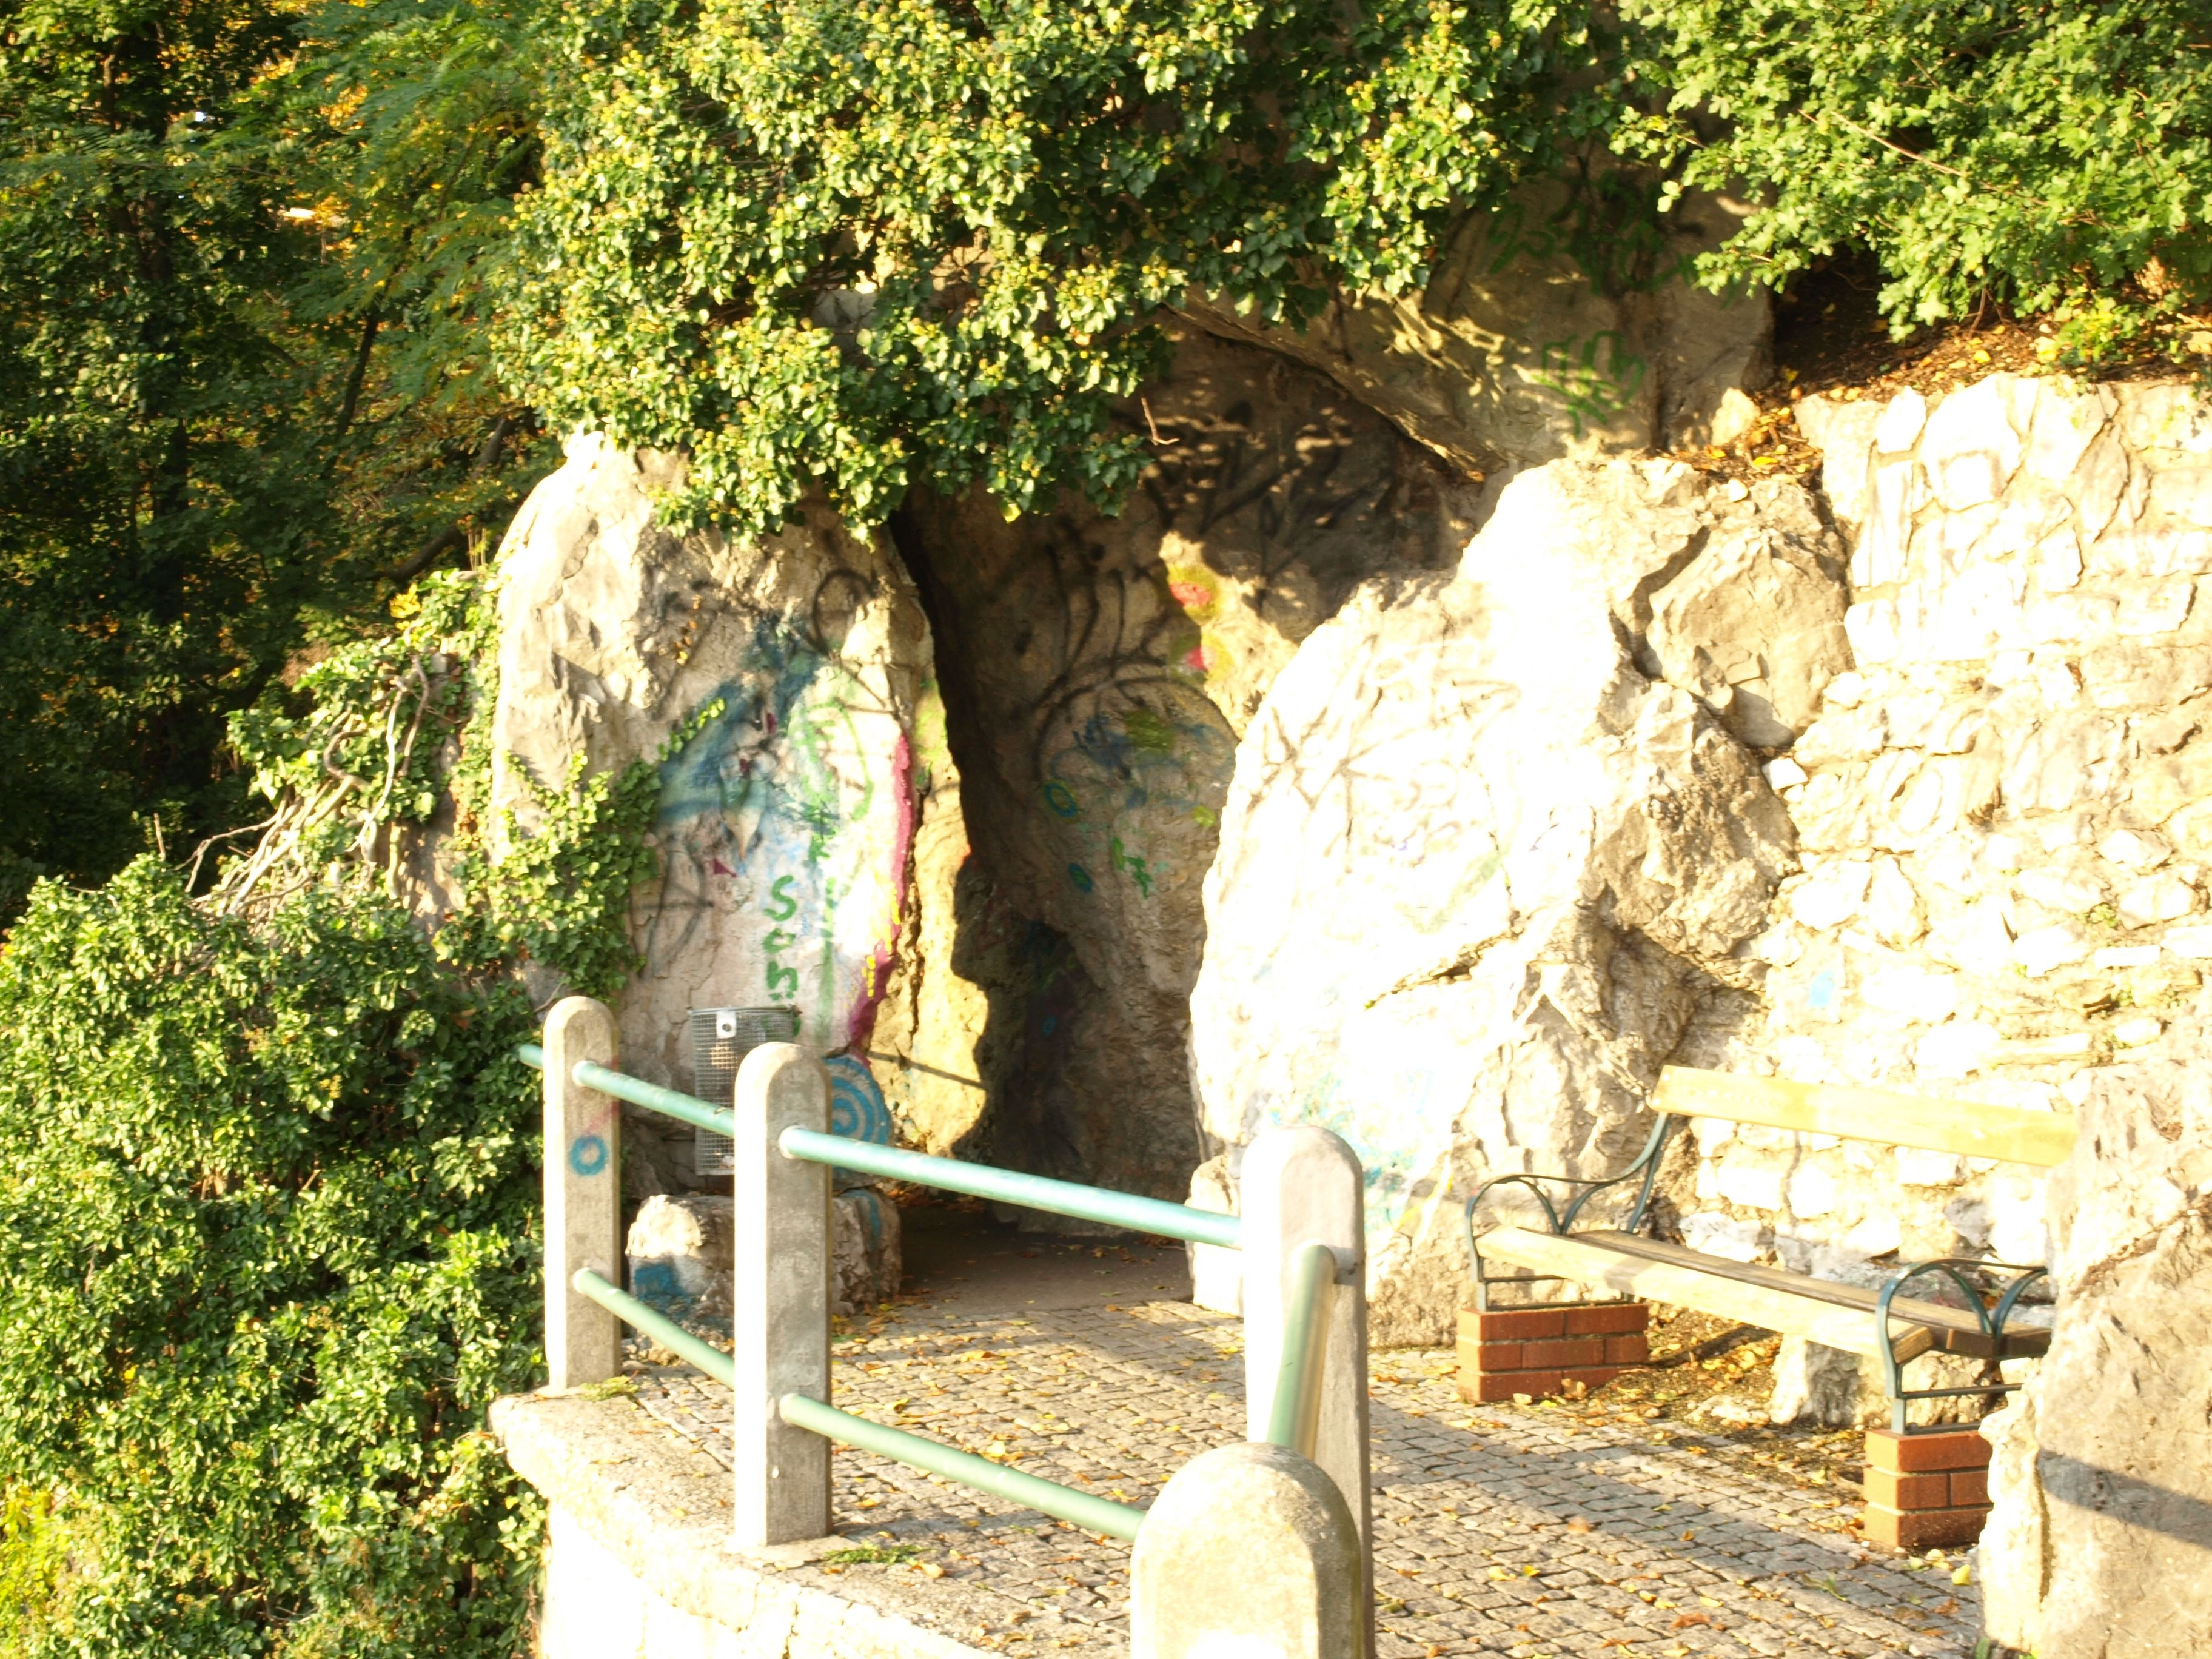
\includegraphics[width=\linewidth]{Image A.jpg}
    \caption{Image A（Fixed）}
  \end{subfigure}
  \begin{subfigure}{0.48\textwidth}
    \centering
    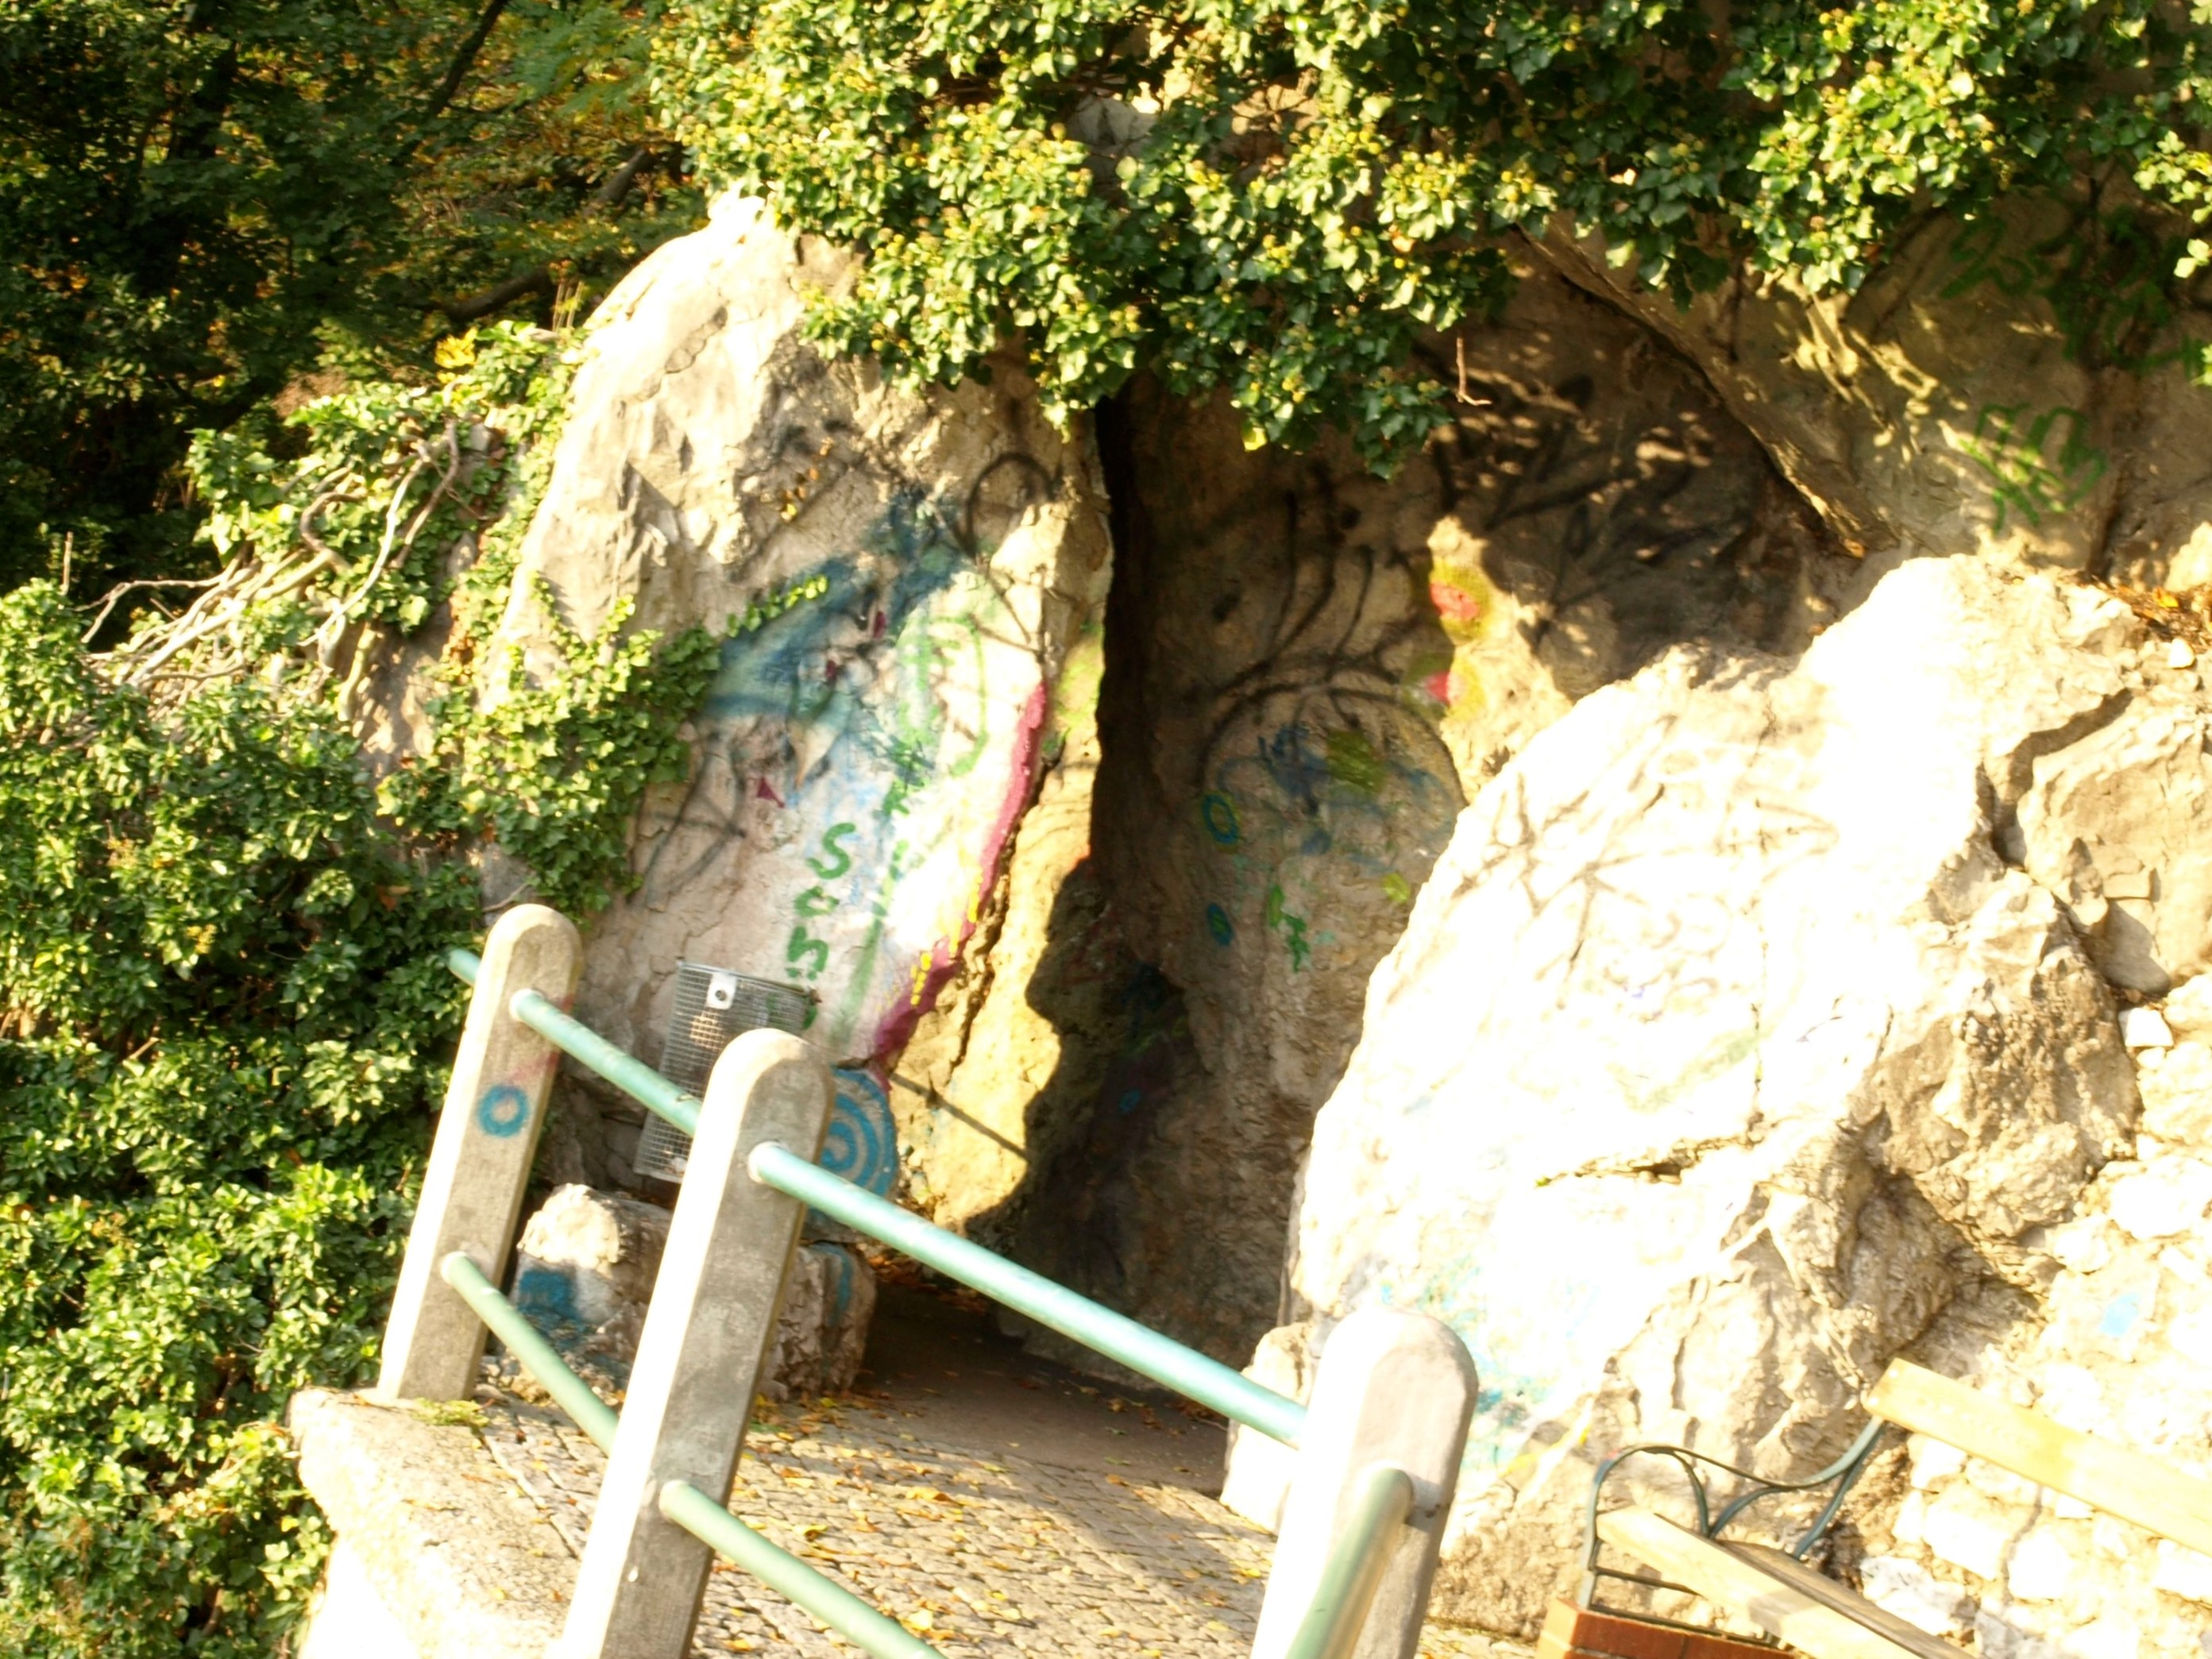
\includegraphics[width=\linewidth]{Image B.jpg}
    \caption{Image B（Moving）}
  \end{subfigure}
  \caption{输入图像}
\end{figure}

\subsection{随机 7 对对应点}
\begin{figure}[H]
  \centering
  \includegraphics[width=0.95\textwidth]{selected_7_points.png}
  \caption{两图随机选取的 7 对对应点（编号一致）}
\end{figure}

\begin{table}[H]
\centering
\caption{7 对对应点坐标}
\begin{tabular}{ccccc}
\toprule
Index & fixed\_x & fixed\_y & moving\_x & moving\_y \\
\midrule
1 & 366.000 & 1681.200 & 106.800 & 1027.200 \\
2 & 1254.528 & 601.344 & 1244.160 & 211.507 \\
3 & 523.144 & 1967.166 & 186.325 & 1343.693 \\
4 & 823.634 & 2513.203 & 335.923 & 1950.843 \\
5 & 982.389 & 1427.300 & 767.398 & 940.585 \\
6 & 758.400 & 940.800 & 675.600 & 411.600 \\
7 & 2324.160 & 362.880 & 2337.984 & 254.016 \\
\bottomrule
\end{tabular}
\end{table}

\subsection{估计得到的单应矩阵}
\begin{equation}
\mathbf{H}=
\begin{bmatrix}
9.6725598367\times10^{-1} & 2.5684774372\times10^{-1} & -1.3077366273\\
-2.5628367296\times10^{-1} & 9.6679783806\times10^{-1} & 7.1632915441\times10^{2}\\
2.3859967617\times10^{-7} & 5.1762999823\times10^{-7} & 1.0000000000
\end{bmatrix}
\end{equation}
该矩阵表示从 \texttt{Image B} 到 \texttt{Image A} 的映射关系。

\subsection{配准结果可视化}
\begin{figure}[H]
  \centering
  \begin{subfigure}{0.48\textwidth}
    \centering
    \includegraphics[width=\linewidth]{registered_B_to_A.png}
    \caption{B 配准到 A}
  \end{subfigure}
  \begin{subfigure}{0.48\textwidth}
    \centering
    \includegraphics[width=\linewidth]{overlay_A_and_registered_B.png}
    \caption{A 与配准后 B 的叠加图}
  \end{subfigure}
  \caption{配准结果}
\end{figure}

\begin{figure}[H]
  \centering
  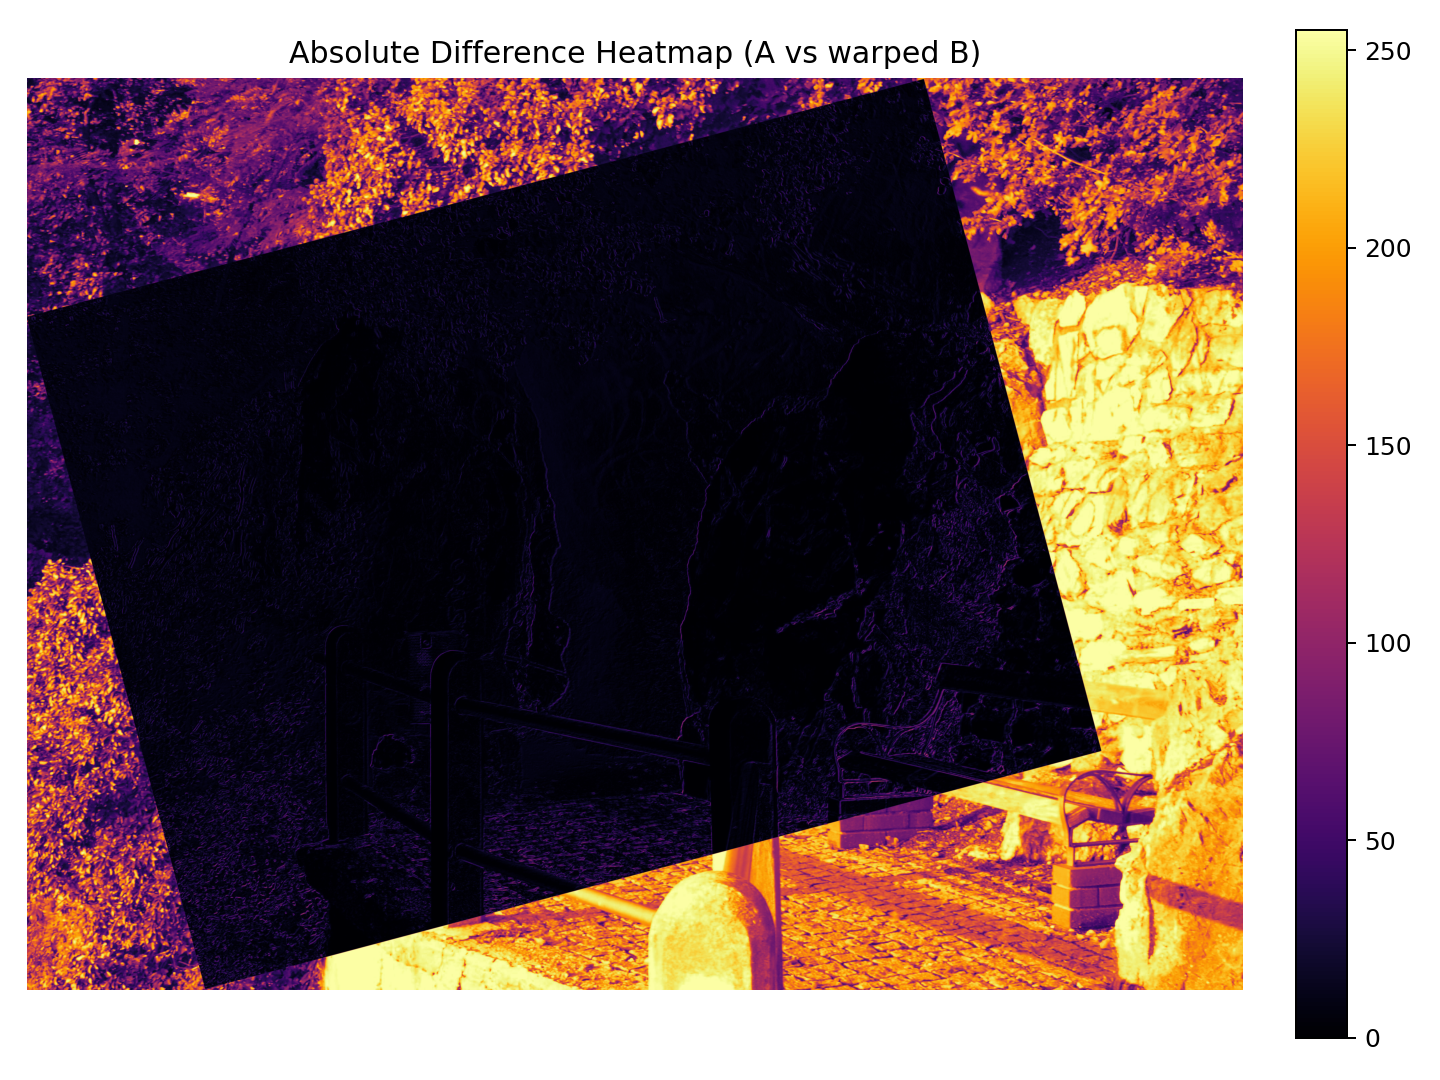
\includegraphics[width=0.7\textwidth]{difference_heatmap.png}
  \caption{绝对差热力图（A 与配准后 B）}
\end{figure}

\subsection{量化指标}
\begin{table}[H]
\centering
\caption{配准指标}
\begin{tabular}{lc}
\toprule
指标 & 数值 \\
\midrule
Raw matched pairs & 1483 \\
RANSAC inliers & 1330 \\
Inlier RMSE & 1.356802 pixels \\
\bottomrule
\end{tabular}
\end{table}

分析：内点数量充足且 RMSE 较小，说明估计的单应矩阵稳定。叠加图中主要结构对齐较好；误差热力图中高误差区域主要来源于视差、遮挡及非平面区域。

\section{结论}
\begin{enumerate}
  \item 本实验完成了从对应点提取到单应矩阵估计、再到图像配准的完整流程。
  \item 在“随机 7 对点 + RANSAC 内点约束”条件下，得到稳定且可用的配准结果。
  \item ORB + RANSAC 方案实现简单、鲁棒性较好，适合本次作业场景。
\end{enumerate}

\section*{附：编译与使用说明}
\begin{itemize}
  \item 建议在 Overleaf 选择 \textbf{XeLaTeX} 编译器。
  \item 上传 \texttt{report\_hw2\_overleaf.tex} 与 \texttt{outputs/} 文件夹（保持目录结构）。
  \item 若同时上传了 \texttt{Image A.jpg} 与 \texttt{Image B.jpg}，可直接显示“原始图像”一节；如不上传，删除该小节即可。
\end{itemize}

\end{document}
